\section{构造 UHF}\label{sec:7-2}

构建良好的通用哈希函数(UHF)的挑战是构建一个使用短密钥实现小碰撞概率的函数。最理想的情况是密钥的长度不取决与被哈希的消息的长度。我们下面给出三种构造。第一种构造是基于算术模运算和多项式的一个\emph{统计性} UHF 的优雅构造。第二种构造基于 \ref{sec:6-4} 节中介绍的 CBC 和级联函数。我们表明,这两者都是\emph{计算性} UHF。第三种构造基于 \ref{sec:6-11} 节中介绍的 $\mathrm{PMAC}_0$。

\subsection{构造 1:使用多项式构建 UHF}\label{subsec:7-2-1}

我们从一个使用多项式模一个素数的 UHF 构造开始。令 $\ell$ 是一个(多项式边界的)长度参数,并令 $p$ 是一个素数。我们定义一个哈希函数 $H_{\rm poly}$,它能将一条消息 $m\in\mathbb{Z}^{\leq\ell}_p$ 哈希为一个单一元素 $t\in\mathbb{Z}_p$。其密钥空间为 $\mathcal{K}:=\mathbb{Z}_p$。

令 $m$ 是一条消息,即 $m=(a_1,\dots,a_v)\in\mathbb{Z}^{\leq\ell}_p$,其中 $0\leq v\leq\ell$。令 $k\in\mathbb{Z}_p$ 是一个密钥。哈希函数 $H_{\rm poly}(k,m)$ 的定义如下:
\begin{equation}\label{eq:7-3}
H_{\rm poly}\big(k,\,(a_1,\dots,a_v)\big)=k^v+a_1k^{v-1}+a_2k^{v-2}+\cdots+a_{v-1}k+a_v\in\mathbb{Z}_p
\end{equation}
也就是说,我们使用 $(1,a_1,a_2,\dots,a_v)$ 作为一个 $v$ 阶多项式 $f(X)$ 的系数向量,然后在一个秘密点 $k$ 处评估 $f(X)$。

这个哈希函数的一个非常有用的特性是,它可以在不提前知道消息长度的情况下进行评估。我们可以随时在消息分组可用时将其输入到哈希函数中。当消息结束时,我们会得到最终的哈希值。我们使用 Horner 的多项式评估方法来实现这一点:

\vspace{5pt}

\hspace*{5pt} 输入:消息 $m=(a_1,\dots,a_v)\in\mathbb{Z}^{\leq\ell}_p$ 和密钥 $k\in\mathbb{Z}_p$\\
\hspace*{26pt} 输出:$t=H_{\rm poly}(k,m)$

\vspace{5pt}

\hspace*{5pt} 1. \quad 置 $t\leftarrow1$\\
\hspace*{26pt} 2. \quad 对于 $i=1,\dots,v$:\\
\hspace*{26pt} 3. \quad\quad\quad 令 $t\leftarrow t\cdot k+a_i\in\mathbb{Z}_p$\\
\hspace*{26pt} 4. \quad 输出 $t$

\vspace{5pt}

\noindent
不难看出,这种算法产生的数值与式 \ref{eq:7-3} 中定义的相同。观察到,对于一条长消息,我们可以使用很少的额外空间来一次处理一个分组。每次迭代都只需要一次乘法和一次加法。
 
在包含多个乘法单元——比如四个——的机器上,我们可以使用 Horner 方法的 $4$ 路并行版本来加快 $H_{\rm poly}$ 的评估速度。假设 $m$ 的长度是 $4$ 的倍数,我们只需将上面的第 $2$ 行和第 $3$ 行替换为以下内容:

\vspace{5pt}

\hspace*{5pt} 2. \quad 对于 $i=1,\dots,v$,每次迭代将 $i$ 递增 $4$:\\
\hspace*{26pt} 3. \quad\quad\quad 令 $t\leftarrow t\cdot k^4+a_i\cdot k^3+a_{i+1}\cdot k^2+a_{i+2}\cdot k+a_{i+3}\;\in\mathbb{Z}_p$

\vspace{5pt}

\noindent
我们可以预先计算 $\mathbb{Z}_p$ 上的 $k_2$,$k_3$ 和 $k_4$。然后,在每次迭代中,我们都并行地执行四个乘法计算来处理四个消息分组。

\begin{snote}[作为一个 UHF 的安全性。]
接下来我们表明,$H_{\rm poly}$ 是一个 ${(\ell/p)}$-UHF。如果 $p$ 是超多项式的,这就意味着 ${(\ell/p)}$ 可忽略不计,也就意味着 $H_{\rm poly}$ 是一个统计性 UHF。
\end{snote}

\begin{lemma}\label{lemma:7-2}
式 \ref{eq:7-3} 中定义的 $(\mathbb{Z}_p,(\mathbb{Z}_p)^{\leq\ell},\mathbb{Z}_p)$ 上的函数 $H_{\rm poly}$ 是一个 ${(\ell/p)}$-UHF。
\end{lemma}

\begin{proof}
考虑 $(\mathbb{Z}_p)^{\leq\ell}$ 中的两条互不相同的消息 $m_0=(a_1,\dots,a_u)$  和 $m_1=(b_1,\dots,b_v)$。我们想要说明 $\Pr[H_{\rm poly} (k,m_0) = H_{\rm poly} (k,m_1)] \leq {\ell/q}$,其中的概率基于从 $\mathbb{Z}_p$ 中随机选择的密钥 $k$。定义 $\mathbb{Z}_p[X]$ 上的两个多项式:
\begin{equation}	\label{eq:7-4}
\begin{aligned}
& f(X):=X^u+a_1X^{u-1}+a_2X^{u-2}+\cdots+a_{u-1}X+a_u\\
& g(X):=X^v+b_1X^{v-1}+b_2X^{v-2}+\cdots+b_{v-1}X+b_v
\end{aligned}
\end{equation}
于是,根据 $H_{\rm poly}$ 的定义,我们需要证明:
\[
\Pr[f(k)=g(k)]\leq{\ell/p}
\]
其中,$k$ 均匀分布在 $\mathbb{Z}_p$ 上。换句话说,我们需要限定使得 $f(k)-g(k)=0$ 成立的点 $k\in\mathbb{Z}_p$ 的数量。由于 $m_0$ 和 $m_1$ 互不相同,所以 $f(X)-g(X)$ 是一个非零的多项式。此外,该多项式最高为 $\ell$ 阶,因此它在 $\mathbb{Z}_p$ 上最多有 $\ell$ 个根。于是,最多有 $\ell$ 个 $k\in\mathbb{Z}_p$ 使得 $f(k)=g(k)$ 成立,因而,对于一个随机的 $k\in\mathbb{Z}_p$,必然有 $\Pr[f(k)=g(k)]\leq{\ell/p}$ 成立,满足要求。
\end{proof}

\begin{snote}[为什么 $H_{\rm poly}(k,m)$ 的首项是 $k^v$?]
在式 \ref{eq:7-3} 中,对 $H_{\rm poly}(k,m)$ 的定义包括一个首项 $k^v$,该项确保该函数是一个适用于变长输入的统计性 UHF。如果我们在定义 $H_{\rm fpoly}(k,m)$ 时不包含该项,即: 
\begin{equation}\label{eq:7-5}
H_{\rm fpoly}\big(k,\,(a_1,\dots,a_v)\big):=a_1k^{v-1}+a_2k^{v-2}+\cdots+a_{v-1}k+a_v\in\mathbb{Z}_p
\end{equation}
那么对于变长输入来说,其结果就不是 UHF。比如说,以下两条消息 $m_0=(a_1,a_2)\in\mathbb{Z}^2_p$ 和 $m_1=(0,a_1,a_2)\in\mathbb{Z}^3_p$ 在所有的密钥 $k\in\mathbb{Z}_p$ 下都是对 $H_{\rm fpoly}$ 的碰撞。尽管如此,在练习 7.16 中,我们将会表明,如果我们把 $H_{\rm fpoly}$ 的输入空间限制在定长的消息上,比如 $\mathcal{M}:=\mathbb{Z}_p^\ell$,那么它仍然是一个统计性 UHF。更具体地说,$H_{\rm fpoly}$ 是一个 $(\ell-1)/p$-UHF。相比之下,式 \ref{eq:7-3} 中定义的函数 $H_{\rm fpoly}$ 对于包含变长输入的输入空间 $\mathbb{Z}_p^\ell$ 来说是一个统计性 UHF。
\end{snote}

\begin{remark}\label{remark:7-1}
函数 $H_{\rm poly}$ 接受 $\mathbb{Z}^{\leq\ell}_p$ 中的输入,并输出 $\mathbb{Z}_p$ 上的值。这并不是十分理想,因为我们更倾向于使用对长为 $n$ 比特的分组进行操作的函数,其中的 $n$ 是某个正整数。我们可以调整式 \ref{eq:7-3} 中对 $H_{\rm poly}$ 的定义,使其不在 $\mathbb{Z}_p$ 上工作,而是在有限域 ${\rm GF}(2^n)$ 上进行算术运算。使用与引理 \ref{lemma:7-2} 完全相同的分析方法,我们可以看到,这个版本的 $H_{\rm poly}$ 是一个 ${(/2^n)}$-UHF。它输出 ${\rm GF}(2^n)$ 上的值。在练习 7.1 中,我们将会表明,简单地将 $H_{\rm poly}$ 定义为模 $2^n$ 运算(即工作在 $\mathbb{Z}_{2^n}$ 上)将得到一个完全不安全的 UHF。
\end{remark}

\begin{snote}[使用 UHF 时的注意事项。]
UHF 可能很脆弱——一个对手如果知道了函数在几个点上的值,就完全有可能回复密钥。例如,$H_{\rm poly}(k,\cdot)$ 在一个点上的值就会完全暴露密钥 $k\in\mathbb{Z}_p$。事实上,如果 $m=(a_1)$,由于 $H_{\rm poly}(k,m)=k+a_1$,那么同时拥有 $m$ 和 $H_{\rm poly}(k,m)$ 的对手立即就能得到 $k\in\mathbb{Z}_p$。因此,在我们对 UHF 的所有应用中,我们都必须始终通过加密或者其他方式向对手隐藏 UHF 的值。
\end{snote}

\begin{snote}[数学细节。]
$H_{\rm poly}$ 的定义需要一个素数 $p$。到目前为止,我们只是假设 $p$ 是一个在最开始时选取的公共值,并且永远固定。在正式的 UHF 框架(见 \ref{subsec:7-1-2} 小节)中,素数 $p$ 是一个系统参数,用 $\Lambda$ 来表示。它由一个\emph{系统参数生成算法} $P$ 生成,该算法将安全参数 $\lambda$ 作为输入,并输出某个素数 $p$。

更确切地说,令 $L:\mathbb{Z}\to\mathbb{Z}$ 是某个将安全参数映射到指定比特长度的素数的函数。那么 $H_{\rm poly}$ 的正式定义应当包括对算法 $P$ 的描述,它将安全参数 $\lambda$ 作为输入,并输出一个长度为 $L(\lambda)$ 的素数 $p$。具体地,$\Lambda:=p$,并且:
\[
\mathcal{K}_{\lambda,p}=\mathbb{Z}_p,
\quad\quad
\mathcal{M}_{\lambda,p}=\mathbb{Z}^{\leq\ell(\lambda)},
\quad\quad
\mathcal{T}_{\lambda,p}=\mathbb{Z}_p
\]
其中 $\ell:\mathbb{Z}\to\mathbb{Z}^{\geq0}$ 是多项式边界的。根据引理 \ref{lemma:7-2},我们可知:
\[
{\rm UHF}\mathsf{adv}[\mathcal{A},H_{\rm poly}](\lambda)\leq{\ell(\lambda)}/{2^{L(\lambda)}}
\]
只要 $2^{L(\lambda)}$ 是超多项式的,上式就是一个 $\lambda$ 的可忽略不计函数。
\end{snote}

\subsection{构造2:CBC 和级联都是计算性 UHF}

接下来,我们表明,\ref{sec:6-4} 节中所定义的 CBC 和级联构造都是计算性 UHF。更一般地,我们表明,任何可扩展的无前缀安全 PRF 都是计算性 UHF。回顾一下,如果对于所有的 $k\in\mathcal{K}$,$x,y\in\mathcal{X}^{\leq\ell-1}$ 和 $a\in\mathcal{X}$,我们都有:
\[
\text{如果}\quad
F(k,x)=F(k,y)
\quad\text{则}\quad
F(k,\;x\,\Vert\,a)=F(k,\;y\,\Vert\,a)
\]
那么定义在 $(\mathcal{K},\mathcal{X}^{\leq\ell},\mathcal{Y})$ 上的 PRF $F$ 就是可扩展的。在上一章中,我们已经证明了 CBC 和级联构造都是无前缀安全 PRF,并且两者都是可扩展的。

\begin{theorem}\label{theo:7-3}
令 $PF$ 是一个定义在 $(\mathcal{K},\mathcal{X}^{\leq\ell+1},\mathcal{Y})$ 上的可扩展的,且无前缀安全的 PRF,其中 $|\mathcal{Y}|$ 是超多项式的,且 $|\mathcal{X}|>1$。那么 $PF$ 也是一个定义在 $(\mathcal{K},\mathcal{X}^{\leq\ell},\mathcal{Y})$ 上的计算性 UHF。
\begin{quote}
特别地,对于每个就 $PF$ 进行攻击游戏 \ref{game:7-1} 的 UHF 对手 $\mathcal{A}$,都必然存在一个无前缀 PRF 对手 $\mathcal{B}$,其中 $\mathcal{B}$ 是一个围绕 $\mathcal{A}$ 的基本包装器,满足:
\end{quote}
\begin{equation}\label{eq:7-6}
{\rm UHF}\mathsf{adv}[\mathcal{A},PF]\leq{\rm PRF^{pf}}\mathsf{adv}[\mathcal{B},PF]+\frac{1}{|\mathcal{Y}|}
\end{equation}
\begin{quote}
此外,$\mathcal{B}$ 只会对 $PF$ 发起两次查询。
\end{quote}
\end{theorem}

\begin{proof}
令 $\mathcal{A}$ 是一个攻击 $PF$ 的 UHF 对手。我们下面构造一个攻击 $PF$ 的无前缀 PRF 对手 $\mathcal{B}$。$\mathcal{B}$ 在攻击游戏 \ref{game:4-2} 中扮演对手,它的目标是区分实验 $0$ 和实验 $1$,在实验 $0$ 中,它用一个随机数 $k\in\mathcal{K}$ 查询一个函数 $f\leftarrow PF(k,\cdot)$,而在实验 $1$ 中,它查询一个随机函数 $f\overset{\rm R}\leftarrow{\rm Funs}[\mathcal{X}^{\leq\ell+1},\mathcal{Y}]$。

首先,我们给出一些关于 $\mathcal{B}$ 如何工作的直觉。$\mathcal{B}$ 从运行 UHF 对手 $\mathcal{A}$ 开始,获得两条不同消息 $m_0,m_1\in\mathcal{X}^{\leq\ell}$。根据 $\mathcal{A}$ 的定义,我们知道,在实验 $0$ 中,我们有:
\[
\Pr[f(m_0)=f(m_1)]={\rm UHF}\mathsf{adv}[\mathcal{A},PF]
\]
而在实验 $1$ 中,由于 $f$ 是一个随机函数,并且 $m_0\neq m_1$,我们有:
\[
\Pr[f(m_0)=f(m_1)]={1}/{|\mathcal{Y}|}
\]
因此,如果 $\mathcal{B}$ 能在 $m_0$ 和 $m_1$ 处查询 $f$,它就能以 $\big\lvert{\rm UHF}\mathsf{adv}[\mathcal{A},PF]-{1}/{|\mathcal{Y}|}\big\rvert$ 的优势区分这两个实验,这就证明了该定理。

不幸的是,对 $\mathcal{B}$ 的这种设计并不奏效,因为 $m_0$ 可能是 $m_1$ 的一个真前缀。在这种情况下,$\mathcal{B}$ 不会被允许在 $m_0$ 和 $m_1$ 处查询 $f$,因为 $\mathcal{B}$ 应当是一个无前缀对手。然而,可扩展的属性提供了一个简单的解决方案:我们可以在 $m_0$ 和 $m_1$ 之后各附加一个分组 $a\in\mathcal{X}$,这样 $m_0\,\Vert\,a$ 就不再是 $m_1\,\Vert\,a$ 的真前缀了。如果 $m_0=(a_1,\dots,a_u)$,$m_1=(b_1,\dots,b_v)$,那么任何的 $a\neq b_{u+1}$ 都能解决这个问题。此外,根据可扩展属性,我们知道:
\[
PF(k,\,m_0)=PF(k,\,m_1)
\quad\Longrightarrow\quad
PF(k,\,m_0\,\Vert\,a)=PF(k,\,m_1\,\Vert\,a)
\]
由于 $m_0\,\Vert\,a$ 不再是 $m_1\,\Vert\,a$ 的真前缀,所以我们的 $\mathcal{B}$ 可以对这两个输入查询 $f$。于是,$\mathcal{B}$ 在区分实验 $0$ 和实验 $1$ 方面就能够获得预期的优势。

更详细地说,$\mathcal{B}$ 的工作流程如下:

\vspace{5pt}

\hspace*{5pt} 运行 $\mathcal{A}$,获得 $\mathcal{X}^{\leq\ell}$ 上的两条互不相同的消息 $m_0$ 和 $m_1$,其中\\
\hspace*{50pt} $m_0=(a_1,\dots,a_u)$,且 $m_1=(b_1,\dots,b_v)$\\
\hspace*{26pt} 假设 $u\leq v$(否则就交换两条消息)\\
\hspace*{26pt} 如果 $m_0$ 是 $m_1$ 的真前缀:\\
\hspace*{50pt} 选择某个 $a\in\mathcal{X}$ 使得 $a\neq b_{u+1}$\\
\hspace*{50pt} 令 $m_0'\leftarrow m_0\,\Vert\,a$,$m_1'\leftarrow m_1\,\Vert\,a$\\
\hspace*{26pt} 否则:\\
\hspace*{50pt} 令 $m_0'\leftarrow m_0$,$m_1'\leftarrow m_1$\\
\hspace*{26pt} // \emph{此时,我们能够确定 $m_0'$不是$m_1'$的真前缀,反之亦然}\\
\hspace*{26pt} 在 $m_0'$ 和 $m_1'$ 处查询 $f$,得到 $t_0:=f(m_0')$ 和 $t_1:=f(m_1')$\\
\hspace*{26pt} 如果 $t_0=t_1$ 则输出 $1$,否则就输出 $0$

\vspace{5pt}

观察到 $\mathcal{B}$ 是一个无前缀 PRF 对手,且只对 $f$ 进行了两次查询,与要求一致。现在,对于 $b=0,1$,令 $p_b$ 是 $\mathcal{B}$ 在实验 $b$ 中输出 $1$ 的概率。那么,在实验 $0$ 中,我们知道:
\begin{equation}\label{eq:7-7}
p_0:=\Pr[f(m_0')=f(m_1')]\geq\Pr[f(m_0)=f(m_1)]={\rm UHF}\mathsf{adv}[\mathcal{A},PF]
\end{equation}
而在实验 $1$ 中,我们知道:
\begin{equation}\label{eq:7-8}
p_1:=\Pr[f(m_0')=f(m_1')]={1}/{|\mathcal{Y}|}
\end{equation}
因此,根据式 \ref{eq:7-7} 和 \ref{eq:7-8},我们有:
\[
{\rm PRF^{pf}}\mathsf{adv}[\mathcal{B},PF]=|p_0-p_1|\geq p_0-p_1\geq{\rm UHF}\mathsf{adv}[\mathcal{A},PF]-{1}/{|\mathcal{Y}|}
\]
由此可得式 \ref{eq:7-6} 成立。
\end{proof}

\begin{snote}[$PF$ 是一个多次查询 UHF。]
引理 \ref{lemma:7-1} 表明,$PF$ 也是一个多次查询 UHF。然而,对该事实的一个直接的证明能够给出一个更好对安全上界。
\end{snote}

\begin{theorem}\label{theo:7-4}
令 $PF$ 是一个定义在 $(\mathcal{K},\mathcal{X}^{\leq\ell+1},\mathcal{Y})$ 上的可扩展的,且无前缀安全 PRF,其中 $|\mathcal{X}|$ 和 $|\mathcal{Y}|$ 都是超多项式的,且 $\ell$ 是多项式边界的。那么 $PF$ 是一个定义在 $(\mathcal{K},\mathcal{X}^{\leq\ell},\mathcal{Y})$ 上的多次查询 UHF。
\begin{quote}
特别地,如果 $|\mathcal{X}|>\ell Q$,那么对于每个 $Q$ 次查询 UHF 对手 $\mathcal{A}$,都必然存在一个 $Q$ 次查询无前缀 PRF 对手 $\mathcal{B}$,其中 $\mathcal{B}$ 是一个围绕 $\mathcal{A}$ 的基本包装器,满足:
\end{quote}
\begin{equation}\label{eq:7-9}
{\rm MUHF}\mathsf{adv}[\mathcal{A},PF]\leq{\rm PRF^{pf}} \mathsf{adv}[\mathcal{B},PF]+\frac{Q^2}{2|\mathcal{Y}|}
\end{equation}
\end{theorem}

\begin{proof}
该证明的证明与定理 \ref{theo:7-3} 的证明相似。对手 $\mathcal{B}$ 首先运行 $Q$ 次查询 UHF 对手 $\mathcal{A}$,以获得 $\mathcal{X}^{\leq\ell}$ 上的几条各不相同的消息 $m_1,\dots,m_s$,其中 $s\leq Q$。接下来,$\mathcal{B}$ 找到一个 $a\in\mathcal{X}$,使得 $a$ 不等于 $m_1,\dots,m_s$ 中的任何一个消息分组。由于 $|\mathcal{X}|$ 是超多项式的,我们可以假设它大于 $\ell Q$,因此这个 $a$ 一定存在。令 $m_i':=m_i\,\Vert\,a$,其中 $i=1,\dots,s$。于是,根据 $a$ 的定义,集合 $\{m_1',\dots,m_s'\}$ 是一个无前缀集合。无前缀对手 $\mathcal{B}$ 现在在 $m_1',\dots,m_s'$ 处向挑战者发起查询,并得到应答 $t_1,\dots,t_s$。如果存在 $i\neq j$ 使得 $t_i=t_j$,$\mathcal{B}$ 就输出 $1$,否则就输出 $0$。

为了分析 $\mathcal{B}$ 的优势,对于 $b=0,1$,我们令 $p_b$ 为 $\mathcal{B}$ 在实验 $b$ 中输出 $1$ 的概率。与式 \ref{eq:7-7} 中一样,可扩展属性意味着:
\[
p_0\geq{\rm MUHF}\mathsf{adv}[\mathcal{A},PF]
\]
在实验 $1$ 中,联合约束意味着:
\[
p_1\leq\frac{Q(Q-1)}{2|\mathcal{Y}|}
\]
因此:
\[
{\rm PRF^{pf}}\mathsf{adv}[\mathcal{B},PF]=|p_0-p_1|\geq p_0-p_1\geq{\rm MUHF}\mathsf{adv}[\mathcal{A},PF]-\frac{Q^2}{2|\mathcal{Y}|}
\]
于是,式 \ref{eq:7-9} 成立。
\end{proof}

\begin{snote}[定理 7.3 和定理 7.4 的应用。]
将定理 \ref{theo:7-4} 应用于 CBC 和级联,可以证明两者都是计算性 UHF。我们在下面的推论中将说明由此产生的误差界限,该界限可由 CBC 定理(定理 \ref{theo:6-3})和级联定理(定理 \ref{theo:6-4})中的界限推出。\footnote{请注意,定理 \ref{theo:7-4} 迫使我们在应用定理 \ref{theo:6-3} 和 \ref{theo:6-4} 时用 $\ell+1$ 来代替 $\ell$。}
\end{snote}

\begin{corollary}\label{cor:7-5}
令 $F$ 是一个定义在 $(\mathcal{K},\mathcal{X},\mathcal{Y})$ 上的安全的 PRF。那么,接受 $\mathcal{X}^{\leq\ell}$ 上的输入的 CBC 构造 $F_{\rm CBC}$(假设 $\mathcal{Y}=\mathcal{X}$ 的大小是超多项式的)和级联构造 $F^*$(假设 $\mathcal{Y}=\mathcal{K}$)对于多项式约束的 $\ell$ 都是计算性 UHF。
\begin{quote}
特别地,对于每个 $Q$ 次查询 UHF 对手 $\mathcal{A}$,必然存在两个无前缀 PRF 对手 $\mathcal{B}_1$ 和 $\mathcal{B}_2$,它们都是 $\mathcal{A}$ 的基本包装器,满足:
\end{quote}
\begin{equation}\label{eq:7-10}
{\rm MUHF}\mathsf{adv}[\mathcal{A},F_{\rm CBC}]\leq{\rm PRF^{pf}}\mathsf{adv}[\mathcal{B}_1,F]+\frac{Q^2(\ell+1)^2+Q^2}{2|\mathcal{Y}|}
\end{equation}
\begin{quote}
和
\end{quote}
\begin{equation}\label{eq:7-11}
{\rm MUHF}\mathsf{adv}[\mathcal{A},F^*]\leq Q(\ell+1)\cdot{\rm PRF^{pf}}\mathsf{adv}[\mathcal{B}_2,F]+\frac{Q^2}{2|\mathcal{Y}|}
\end{equation}
\end{corollary}

\noindent
在式 \ref{eq:7-10} 和 \ref{eq:7-11} 中令 $Q:=2$,可以得到作为 UHF 的 $F_{\rm CBC}$ 和 $F^*$ 的误差上界。

\subsection{构造 3:使用小的 PRF 构建的一种并行 UHF}\label{subsec:7-2-3}

CBC 和级联构造都能从小领域的 PRF 中产生高效的 UHF,但是它们本身都是串行性的,因而无法利用硬件的并行性。幸运的是,从一个小领域的 PRF 中构造一个适用于并行架构的 UHF 并不困难。一个被称为异或哈希(XOR-hash)的例子,用$F^\oplus$ 表示,如图 \ref{fig:7-2} 所示。异或哈希定义在 $(\mathcal{K},\mathcal{X}^{\leq\ell},\mathcal{Y})$ 上,其中 $\mathcal{Y}=\{0,1\}^n$,并且是由一个定义在 $(\mathcal{K},\mathcal{X}\times\{1,\dots,\ell\},\mathcal{Y})$ 上的 PRF $F$ 构建来的。异或哈希的工作方式如下:

\begin{figure}
  \centering
  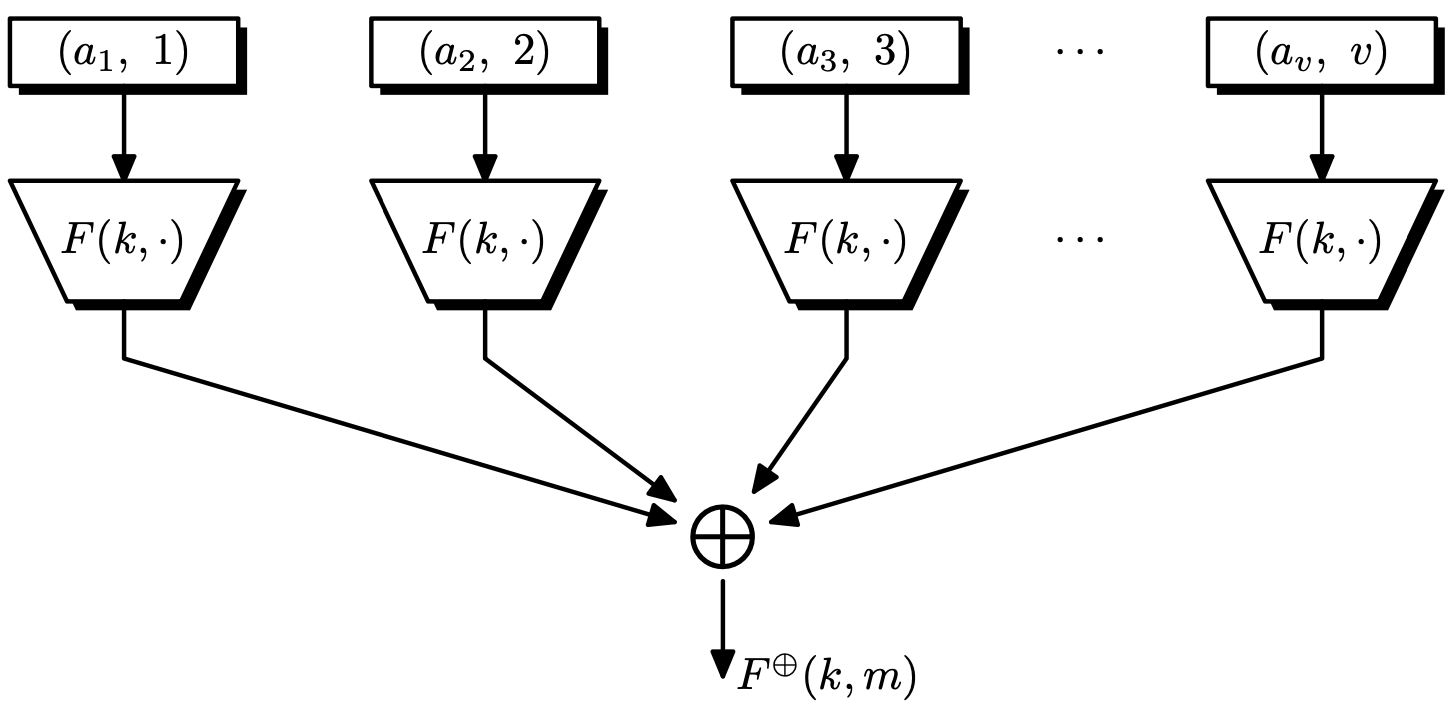
\includegraphics[width=0.65\linewidth]{figures/chapter7/fig2.png}
  \caption{一个来自小 PRF 的并行 PRF}
  \label{fig:7-2}
\end{figure}

\vspace{5pt}

\hspace*{5pt} 输入:$k\in\mathcal{K}$ 和 $m=(a_1,\dots,a_v)\in\mathcal{X}^{\leq\ell}$,其中 $0\leq v\leq\ell$\\
\hspace*{26pt} 输出:一个 $\mathcal{Y}$ 中的标签

\vspace{5pt}

\hspace*{5pt} 令 $t\leftarrow0^n$\\
\hspace*{26pt} 对于 $i=1,\dots,v$:\\
\hspace*{50pt} 令 $t\leftarrow t\oplus F(k,\,(a_i,i))$\\
\hspace*{26pt} 输出 $t$

\vspace{5pt}

\noindent
对 $F^\oplus$ 的评估可以很容易地以并行的方式完成。下面的定理表明,$F^\oplus$ 是一个计算性 UHF。请注意,与我们之前介绍的 UHF 构造不同,$F^\oplus$ 的安全性不取决于输入消息的长度。在下一节中,我们将使用 $F^\oplus$ 来构建一个适用于并行架构的安全的 MAC。

\begin{theorem}\label{theo:7-6}
令 $F$ 是一个安全的 PRF,并且 $|\mathcal{Y}|$ 是超多项式的。那么 $F^\oplus$ 是一个计算性 UHF。
\begin{quote}
特别地,对于每个 UHF 对手 $\mathcal{A}$,都必然存在一个 PRF 对手 $\mathcal{B}$,其中 $\mathcal{B}$ 是一个围绕 $\mathcal{A}$ 的基本包装器,满足:
\end{quote}
\begin{equation}\label{eq:7-12}
{\rm UHF}\mathsf{adv}[\mathcal{A},F^\oplus]\leq{\rm PRF}\mathsf{adv}[\mathcal{B},F]+\frac{1}{|\mathcal{Y}|}
\end{equation}
\end{theorem}

\begin{proof}
该证明是一个由两个游戏组成的序列。

\vspace{5pt}

\noindent\textbf{游戏 $\mathbf{0}$}。
该游戏的挑战者计算:

\vspace{5pt}

\hspace*{5pt} 选取 $k\overset{\rm R}\leftarrow\mathcal{K}$,令 $f\leftarrow F(k,\cdot)$

\vspace{5pt}

\noindent
对手输出 $\mathcal{X}^{\leq\ell}$ 中的两条互不相同的消息 $U$ 和 $V$。令 $u:=|U|$,$v:=|V|$。定义 $W_0$ 为在游戏 $0$ 中,条件:
\begin{equation}\label{eq:7-13}
\bigoplus_{i=0}^{u-1}f(U[i],i)=\bigoplus_{j=0}^{v-1}f(V[j],j)
\end{equation}
成立的事件。显然,我们有:
\begin{equation}\label{eq:7-14}
\Pr[W_0]={\rm UHF}\mathsf{adv}[\mathcal{A},F^\oplus]
\end{equation}

\noindent\textbf{游戏 $\mathbf{1}$}。
我们打出``PRF牌",将挑战者的计算修改为:

\vspace{5pt}

\hspace*{5pt} 选取 $f\overset{R}\leftarrow{\rm Funs}[\mathcal{X}\times\{1,\dots,\ell\},\mathcal{Y}]$

\vspace{5pt}

\noindent
我们定义 $W_1$ 为在游戏 $1$ 中,式 \ref{eq:7-13} 中的条件成立的事件。

同之前一样,存在一个 PRF 对手 $\mathcal{B}$ 使得:
\begin{equation}\label{eq:7-15}
\big\lvert\Pr[W_0]-\Pr[W_1]\big\rvert\leq{\rm PRF}\mathsf{adv}[\mathcal{B},F]
\end{equation}

\noindent
证明的关键在于约束 $\Pr[W_1]$,即约束式 \ref{eq:7-13} 对消息 $U$ 和 $V$ 成立的概率。不妨假设 $u\geq v$,并在必要时调换 $U$ 和 $V$。不难发现,由于 $U$ 和 $V$ 是互不相同的两条消息,那么一定存在一个索引 $i^*$,使得式 \ref{eq:7-13} 中左侧的数对 $(U[i^*],i^*)$ 不会出现在右侧的数对 $(V[j],j)$ 中:如果 $u>v$,那么令 $i^*=u-1$ 即可完成任务;否则,如果 $u=v$,那么一定存在某个 $i^*$,使得 $U[i^*]\neq V[i^*]$,那么该 $i^*$ 就能完成任务。

我们可以将式 \ref{eq:7-13} 改写为:
\begin{equation}\label{eq:7-16}
f(U[i^*],i^*)=\bigoplus_{i\neq i^*}f(U[i],i)\ \ \oplus\ \ \bigoplus_jf(V[j],j)
\end{equation}
由于式 \ref{eq:7-16} 的左右两侧相互独立,并且左侧均匀分布在 $\mathcal{Y}$ 上,所以等号成立的概率为 ${1}/{|\mathcal{Y}|}$。由此可得:
\begin{equation}\label{eq:7-17}
\Pr[W_1]={1}/{|\mathcal{Y}|}
\end{equation}
于是,根据式 \ref{eq:7-14},\ref{eq:7-15} 和 \ref{eq:7-17},定理得证。
\end{proof}

在练习 7.27 中,我们将对定理 \ref{theo:7-6} 进行推广,得到 $F^\oplus$ 作为一个多次查询 UHF 的约束。